
\subsection{Experiments on effects of orderings}
\label{s.ilu}
In the idea of mixing the preconditioning and AD discussed in~\secref{s.precond},
the ILU preconditioning is computed using the natural ordering of the given matrix. However,
it is a well-known fact that the number of fill-ins is heavily dependent on the ordering.
So, we can improve the number of fill-ins by carefully choosing an ordering.
On the other hand, we compute the Jacobian matrix by AD techniques in which
the matrix computed in a particular ordering. We need a reformulation to
fit these two computations from ILU preconditioning and the automatic differentiation.

As we discussed in the iterative solvers, like BICGSTAB,
we always need to have a matrix-vector product like $Az$.
This suits the AD behavior which gets a seed matrix, here the vector $z$, and
computes the matrix-vector product.
A reordering of the matrix for ILU preconditioning
needs a consideration also in the seed matrix.
Without reordering, a preconditioning would look like as,
$$
Ax = b \rightarrow M^{-1} Ax = M^{-1}b.
$$
We would add the reordering to this equation results in the following equations,
\begin{align*}
Ax = b \rightarrow M^{-1} Ax &= M^{-1}b\\
P^T M^{-1} P P^T A P P^T x &= P^T M^{-1} P P^T b\\
(P^T M^{-1} P) (P^T A P) P^T x &= (P^T M^{-1} P) P^T b\\
(P^T M P)^{-1} (P^T A P) P^T x &= (P^T M P)^{-1} P^T b\\
\tilde{M}^{-1}\tilde{A}\tilde{x} &= \tilde{M}^{-1}\tilde{b}.
\end{align*}
As this equation shows, we need a reordering in the matrix $A$ if we
have the reordering in the preconditioner.
So, the matrix-vector product $\tilde{A}.\tilde{x} = P^T A P x$
should be computed instead of $A.x$.

Let the function $ad$ to compute the automatic differentiation
and the function $bicgstab$ to compute a step of BICGSTAB iterative solver,
we modify the seed matrix and the return result of this function
to adapt the reordering as follows,
\begin{align*}
z &= P \tilde{x}\\
APz &= ad(f,z,...)\\
\tilde{x} &= bicgstab(P^T APz,...)
\end{align*}
in which the seed matrix $P \tilde{x}$ is used instead of $x$.
After computation of AD, the resulting matrix-vector product $APz$,
should be multiplied by $P^T$ from the left before continuing by the
computations regarding BICGSTAB.

Here, we investigate the preconditioning based on the incomplete LU factorization (ILU) \cite{ilu2003}.
Between different models of ILU, we consider the level-based ILU factorization here.
We use a graph model for ILU instead of the current matrix model to have a unified
work on graphs in the implemented library. This graph model is based on the proposed
model in ~\cite{precond-pothen}. If the given matrix is nonsymmetric,
we put a vertex for each row. We also connect the vertex $i$ to the
vertex $j$ with a directed edge if the corresponding element $(i,j)$ in matrix
in nonzero. If the matrix is symmetric, these edges are undirected. This means
the graph is a simple graph and the given matrix is the adjacency
matrix of the graph.
Now, we look at the effects of preordering for the vertices of the given preconditioning graph to reduce fill-ins in ILU factorization. Later, we would study further how this fill-in reduction increases the additionally required elements.

As same as coloring algorithms, finding an ILU factorization with the minimum
fill-ins is also an NP-complete problem. There are a lot of literature
considering this problem\cite{ilu_ordering1,ilu_ordering2,ilu_ordering3,ilu_ordering4}.
Again, the ILU factorization is computed in a specific order which is essential
in the minimum fill-ins. Here we bring an example to show how the order affects
the ILU factorization and the number of fill-ins.
For example, let's consider first the following matrix,
$$\begin{bmatrix}
1 & 1 & 0 & 1 & 0 & 1 & 0\\
1 & 1 & 1 & 0 & 0 & 0 & 0\\
0 & 1 & 1 & 0 & 1 & 0 & 1\\
1 & 0 & 0 & 1 & 1 & 0 & 0\\
0 & 0 & 1 & 1 & 1 & 1 & 1\\
1 & 0 & 0 & 0 & 1 & 1 & 1\\
0 & 0 & 1 & 0 & 1 & 1 & 1\\
\end{bmatrix}.$$

We set up a graph for ILU preconditioning.
The graph for preconditioning would be an undirected graph
since the matrix is symmetric.
For example, the graph in Figure~\ref{bad_order_fillin}
is computed from the previous matrix. Here, we illustrated the
computation of Cholesky factorization step by step.
Figure~\ref{bad_order_fillin} computes the Cholesky factorization
in which the order of vertices are the numbering written on the vertices
as labels. The ordering in Figure~\ref{bad_order_fillin} is a worst-case ordering that produces $6$ fill-ins. These fill-ins are illustrated as dotted lines.

%\begin{figure}
%\centering
% 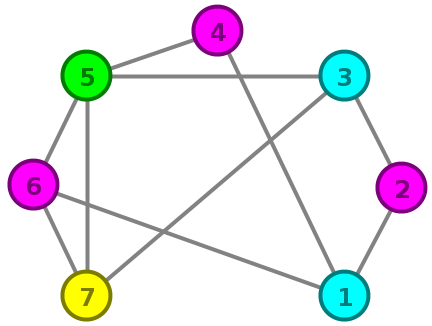
\includegraphics[width=0.45\linewidth]{bad_order_color}
% \hfill
% 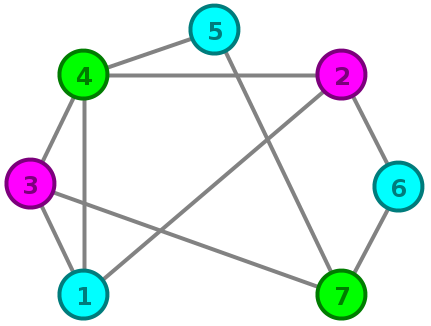
\includegraphics[width=0.45\linewidth]{good_order_color}
%\end{figure}

\begin{figure}
\centering
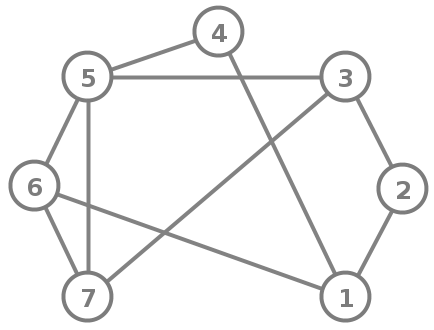
\includegraphics[width=0.28\linewidth]{bad_order}
\hfill
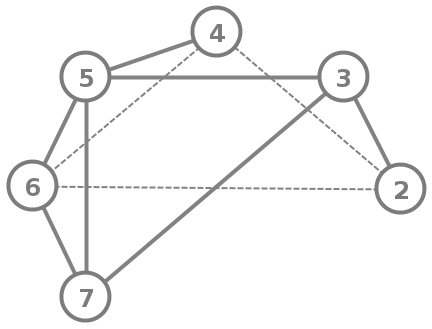
\includegraphics[width=0.28\linewidth]{bad_order_1_removed}
\hfill
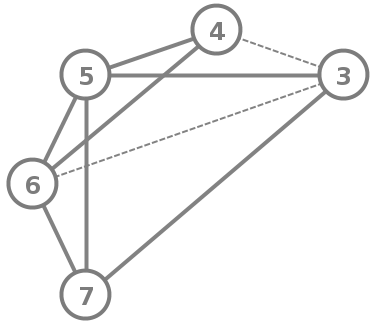
\includegraphics[width=0.23\linewidth]{bad_order_2_1_removed}
\hfill
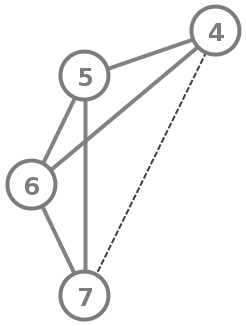
\includegraphics[width=0.16\linewidth]{bad_order_3_2_1_removed}
\caption{A worst case ordering generates $6$ fill-ins. The ordering here is the
numbering which visualized as labels.}
\label{bad_order_fillin}
\end{figure}

Figure~\ref{good_order_fillin} shows how the new ordering produces
$5$ fill-ins when the ordering is $2, 3, 4$. However, the best ordering produces only $3$ fill-ins
as Figure~\ref{good_order_fillin2} shows when the ordering is $2, 5, 3$.

\begin{figure}
\centering
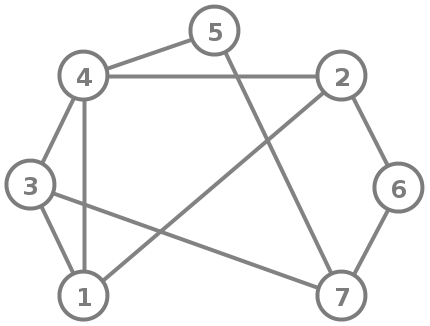
\includegraphics[width=0.28\linewidth]{good_order}
\hfill
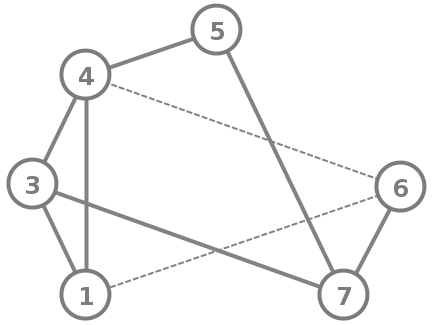
\includegraphics[width=0.28\linewidth]{good_order_2_removed}
\hfill
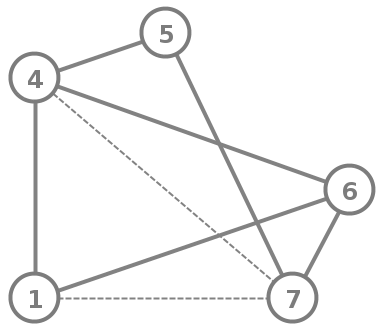
\includegraphics[width=0.23\linewidth]{good_order_3_2}
\hfill
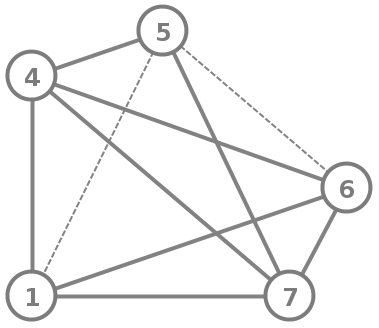
\includegraphics[width=0.16\linewidth]{good_order_4_3_2}
\caption{The order of elimination $2, 3, 4$ generates $5$ fill-ins.}
\label{good_order_fillin}
\end{figure}


\begin{figure}
\centering
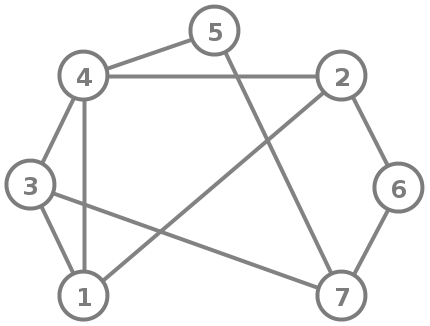
\includegraphics[width=0.27\linewidth]{good_order}
\hfill
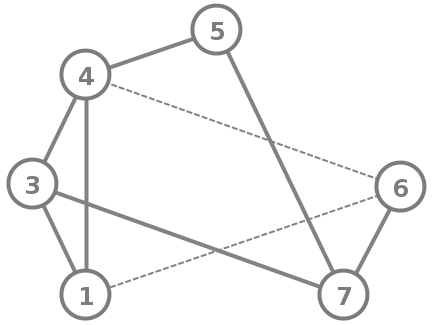
\includegraphics[width=0.27\linewidth]{good_order_2_removed}
\hfill
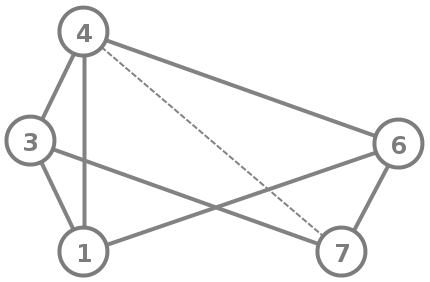
\includegraphics[width=0.23\linewidth]{good_order_5_2_removed}
\hfill
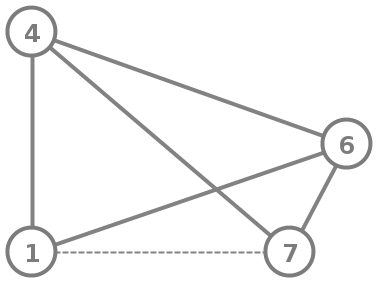
\includegraphics[width=0.18\linewidth]{good_order_3_5_2_removed}
\caption{The order of elimination $2, 5, 3$ generates $3$ fill-ins.}
\label{good_order_fillin2}
\end{figure}

There are various ordering which were studied for coloring heuristics
throughout years.
As we discussed in the previous section, there are different ordering for coloring
like \textit{LFO}, \textit{IDO}, and \textit{SLO}.
%Here, we have a list of such orderings for coloring
%which is available in \textit{PreCol}.
%In each item, we explain how the algorithm selects the next vertex.
%\begin{itemize}
%\item Largest-First Ordering (LFO)~\cite{LFO} chooses a vertex with minimum degree in each step.
%\item Incidence-degree Ordering (IDO)~\cite{IDO} chooses first the vertex with maximum degree in $G$, namely $v$. Then, it selects the %matrix with the maximal degree in the subgraph induced by $V(G)-v$. It means the vertex with the maximum incidence degree is selected.
%\item Saturation-degree Ordering (SDO)~\cite{SDO} chooses first the vertex with the maximum degree in $G$, namely $v$. Then, it chooses the vertex with the maximum saturation degree in
%$V$. The saturation degree of the vertex $v$ is the number of different colored vertices in the neighbors of $v$.
%\end{itemize}
In addition to these orderings, we consider three other orderings for preconditioning:
\begin{itemize}
\item Natural Ordering (Nat): This is the natural ordering of the input matrix.
\item Minimum Degree Ordering (Min): The one generates a list of vertices which are sorted based on the degree from minimum to maximum.
\item Metis Ordering\cite{metis,par-nested-disection} (Metis):
This is a fill-reducing ordering based on the algorithm of nested dissection. We use the software \textit{Metis} for generating this ordering.
\end{itemize}
The Table~\ref{ilu-effect} shows how different ordering generates different fill-ins required elements.
The number of fill-ins compared based on the different orderings
for the graph vertices. The number of colors remains the same since we change only the ordering for
ILU factorization.
The left table is the computation for the matrix \textit{nos3.mtx}
and the right one is the computation for the matrix \textit{gyro\_m}.
Both are from the Florida sparse matrix collections.
\begin{table}
\begin{tabular}{|c|c|c|c|c|}
\hline250
Orders & Colors & Fill-ins\\\hline
Nat & 15 & 70\\\hline
Min & 15 & 52\\\hline
Metis & 15 & 52\\\hline
\end{tabular}
\hfill
\begin{tabular}{|c|c|c|c|c|}
\hline
Orders & Colors & Fill-ins \\\hline
Nat & 34 & 8760 \\\hline
Min & 34 & 8414 \\\hline
Metis & 34 & 642\\\hline
\end{tabular}
\caption{The number of fill-ins compared based on the different orderings
for the graph vertices. The number of colors remains the same since we change only the ordering for
ILU factorization.
The left table is the computation for the matrix \textit{nos3.mtx}
and the right one the computation is for the matrix \textit{gyro\_m}.
Both are from the Florida sparse matrix collections.}
\label{ilu-effect}
\end{table}

The computation are carried out on the matrices \textit{nos3.mtx}
and the matrix \textit{gyro\_m} from
the Florida sparse matrix collections. The block size is
chosen to be $50$ for the matrix \textit{gyro\_m} and $15$ for
the matrix \textit{nos3}. Also, the coloring algorithm is an one-sided
restricted coloring. In this table, the fill-reducing Metis ordering
generates the minimum fill-in.
Another observation is that the Metis and Min ordering are generating almost the same
number of fill-ins for the small matrices.
It is only for the big matrices which the efficiency of Metis ordering is visible.

This difference in the number of fill-ins can affect the convergence speed
relatively. Both Figure~\ref{nat_convergence}
and Figure~\ref{metis_convergence} show
the convergence history of the BICGSTAB solvers on the matrix \textit{nos3}.
The three line charts are the convergence history of the solver with
no preconditioning, ILU preconditioning with block-diagonal sparsification,
and ILU preconditioning with block-diagonal sparsification together with the found
additionally required elements, respectively.
Here, the block size is chosen to be $10$ and the level of ILU factorization
is $10$.
Clearly, Figure~\ref{metis_convergence} has a better convergence rate in the chart
in which the additionally required elements are added in comparison with the same
chart in Figure~\ref{nat_convergence}.

\begin{figure}
\centering
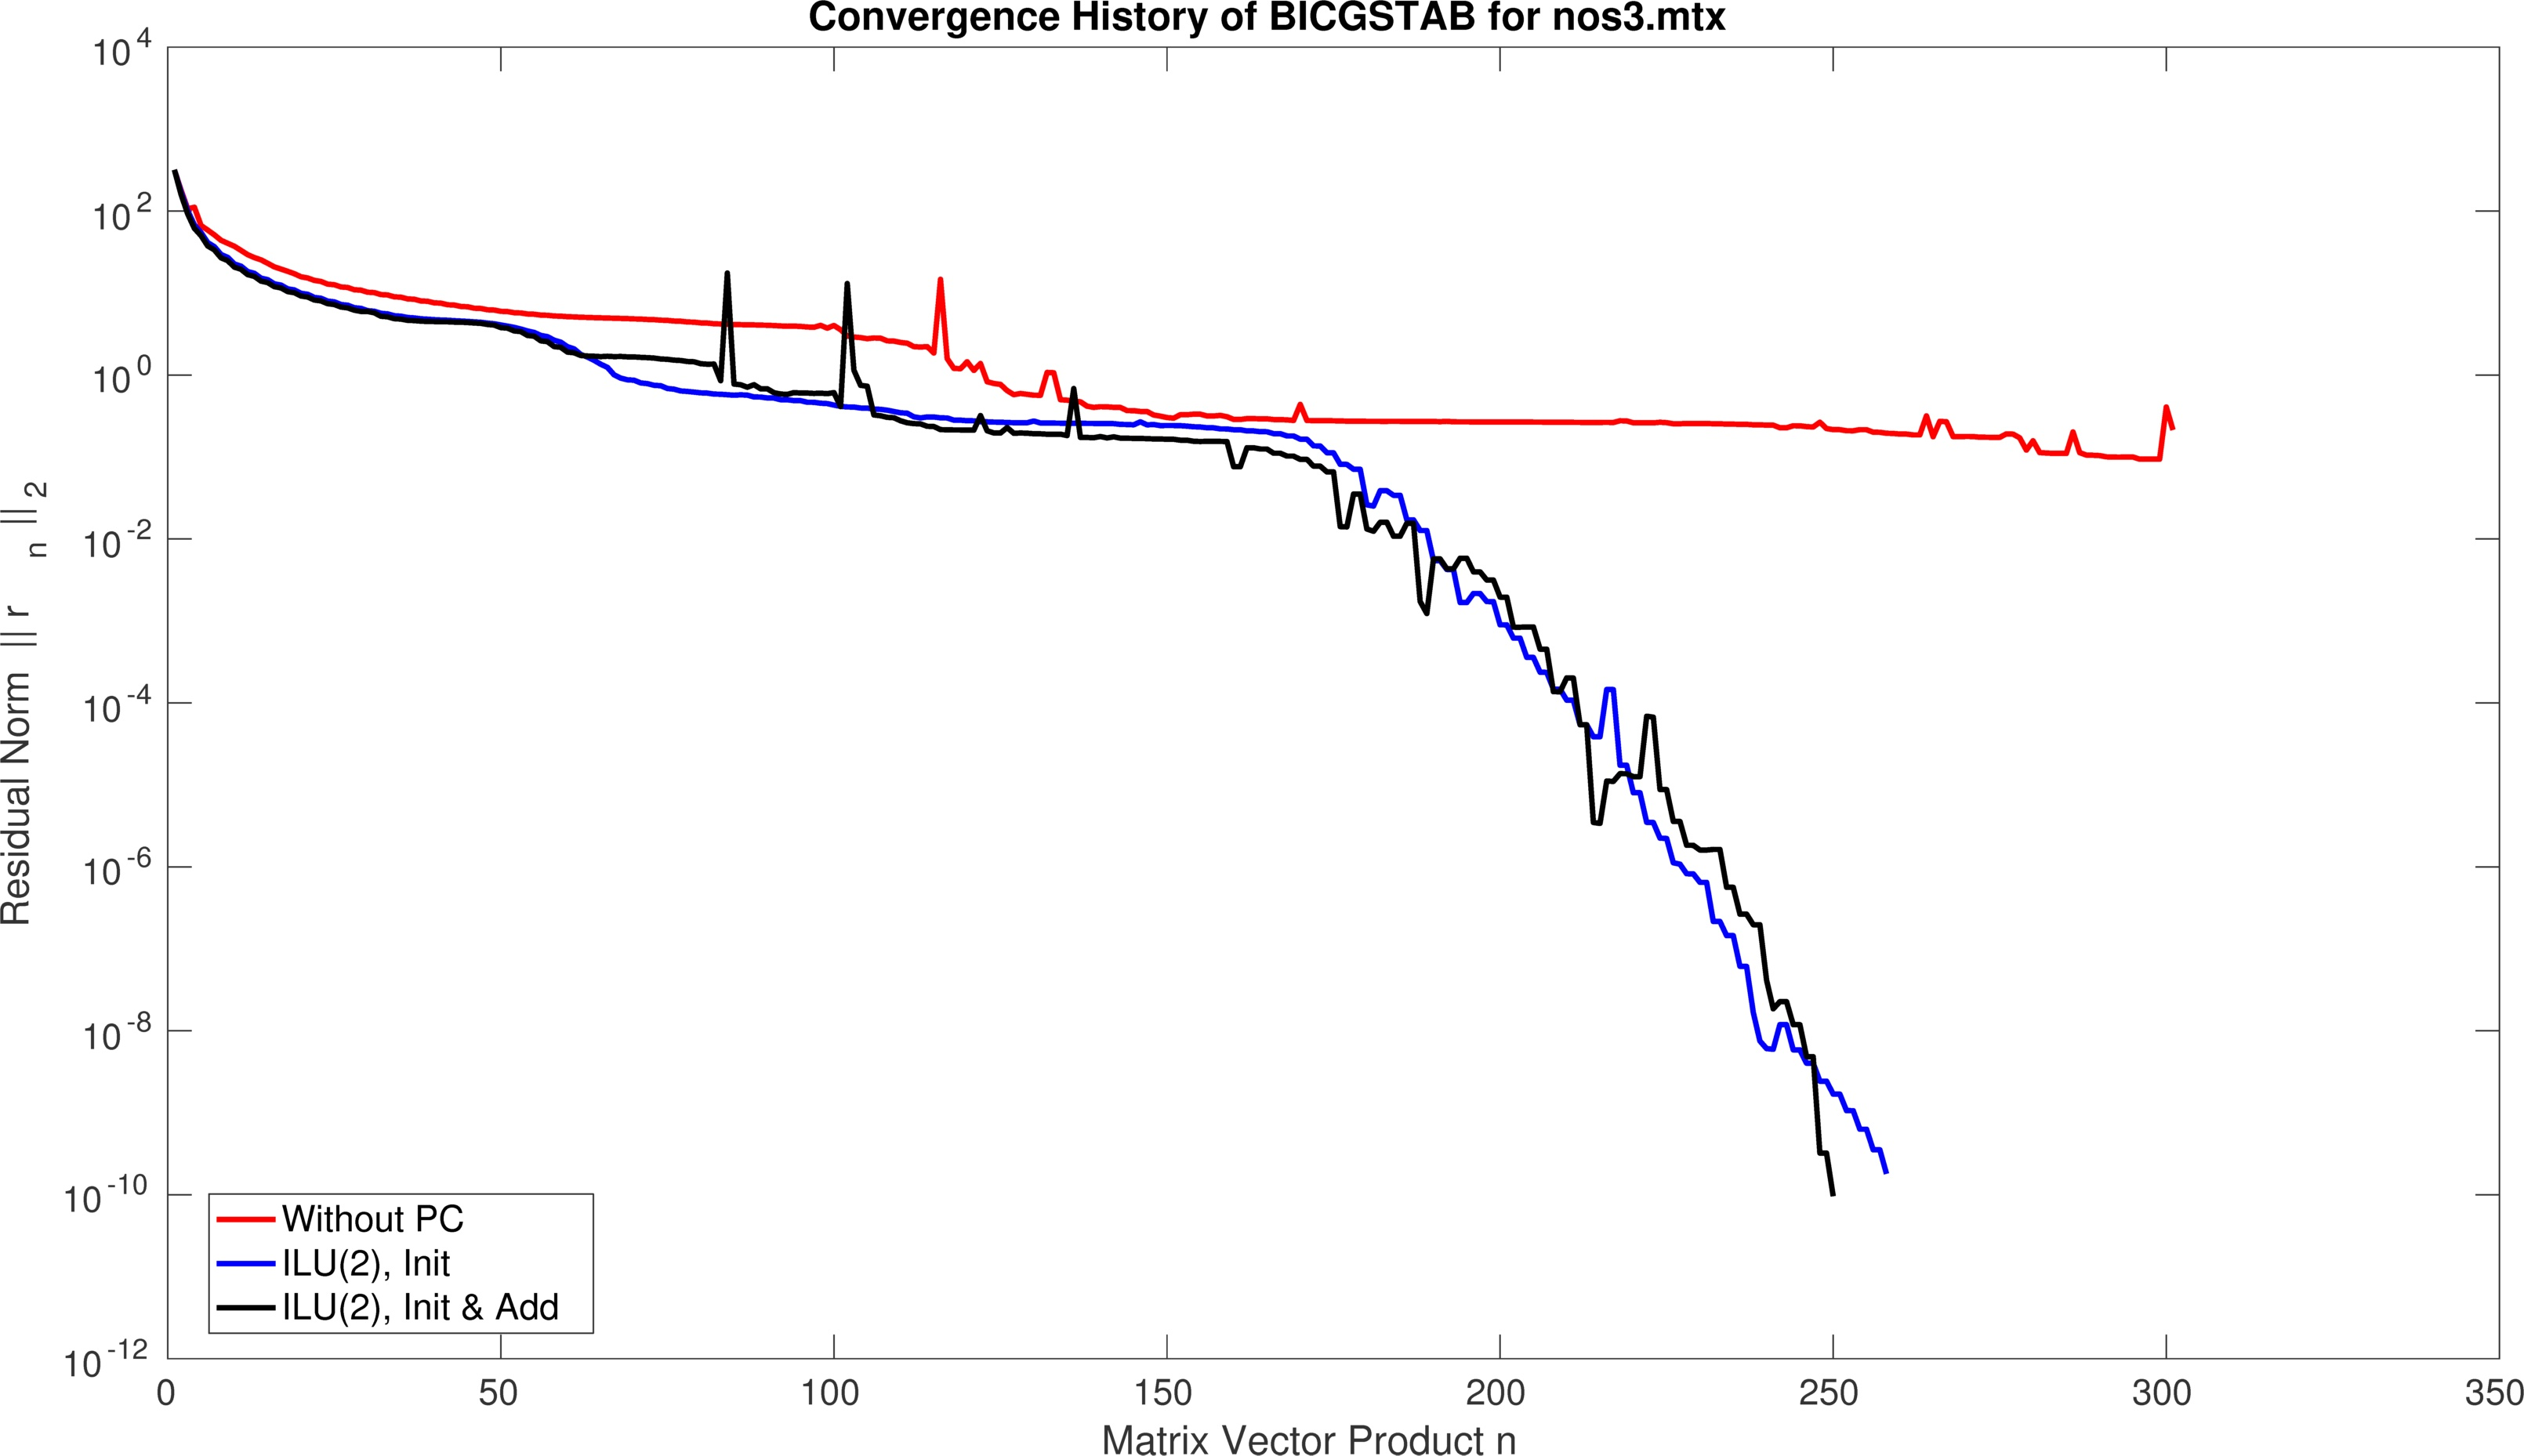
\includegraphics[width=0.9\linewidth]{nos3_mtx_convergence_nat}
\caption{Natural ordering results in a worst convergence.}
\label{nat_convergence}
\end{figure}
\begin{figure}
\centering
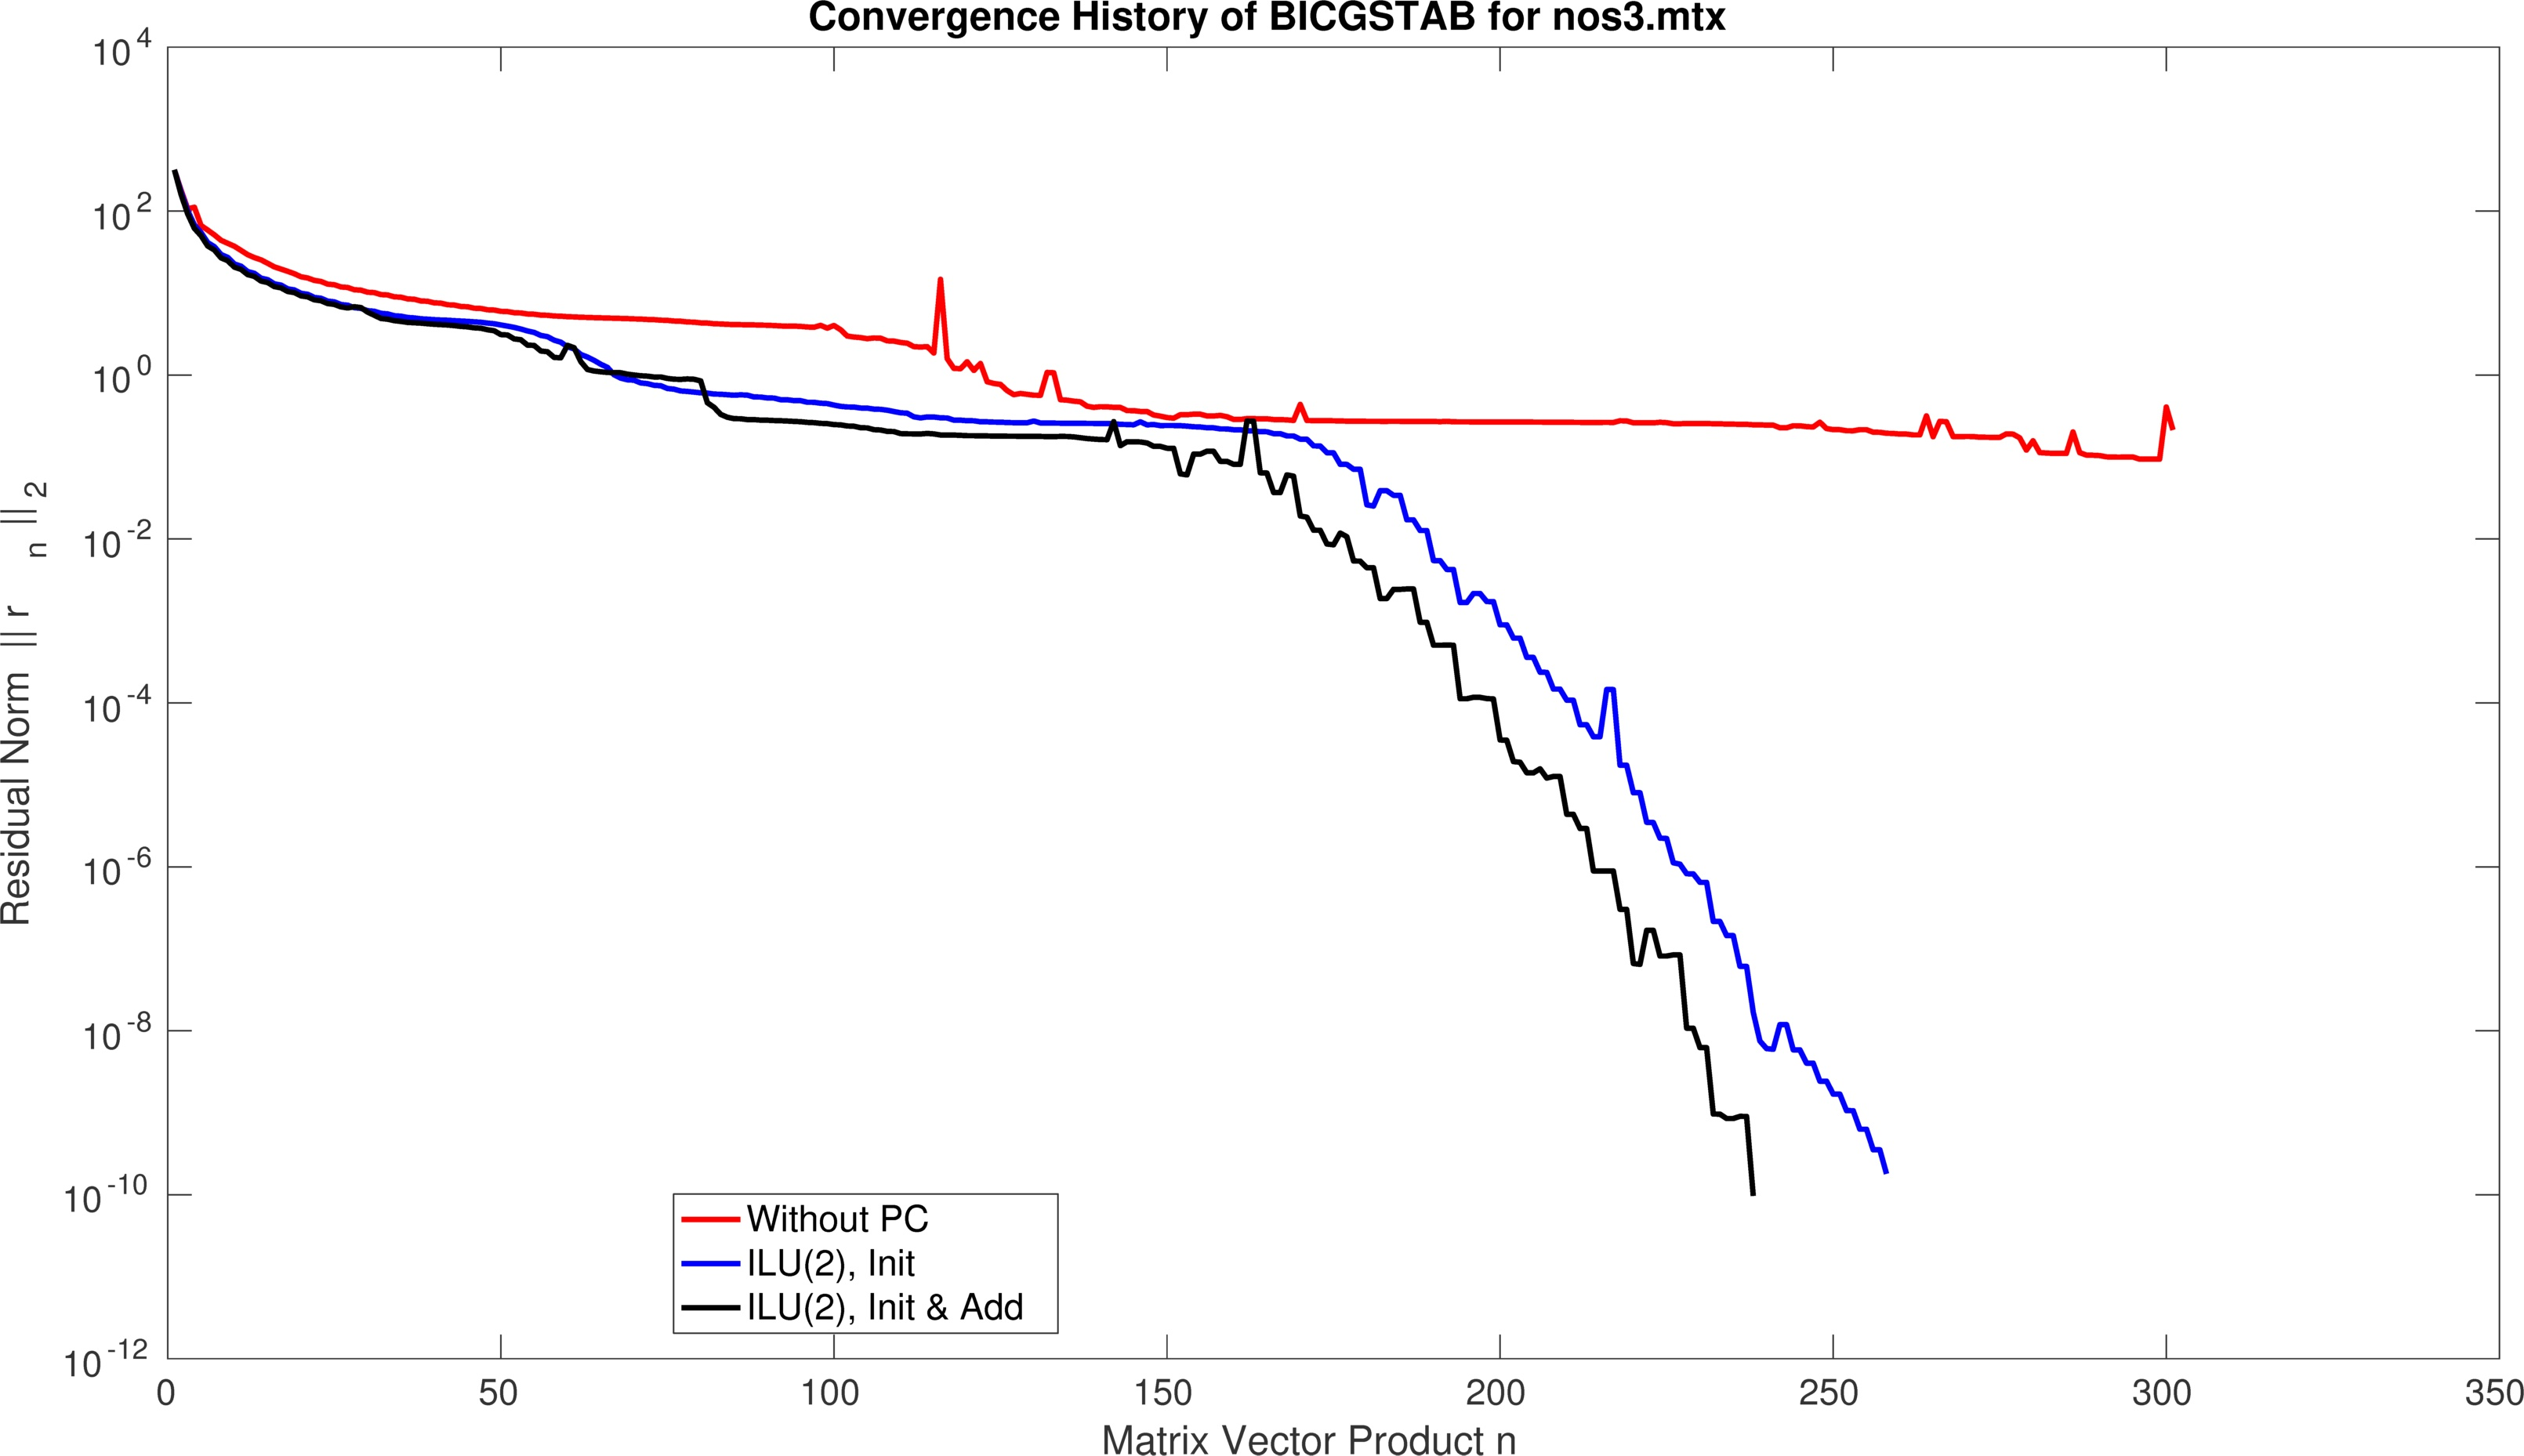
\includegraphics[width=0.9\linewidth]{nos3_mtx_convergence_metis}
\caption{Metis ordering results in a better convergence.}
\label{metis_convergence}
\end{figure}

So far, we decided for the level of ILU factorization arbitrarily.
Here, we want to see the actual influence of the level parameter on
the fill-ins which is visualized in \figref{el_fillins_orderings},
\begin{figure}
\centering
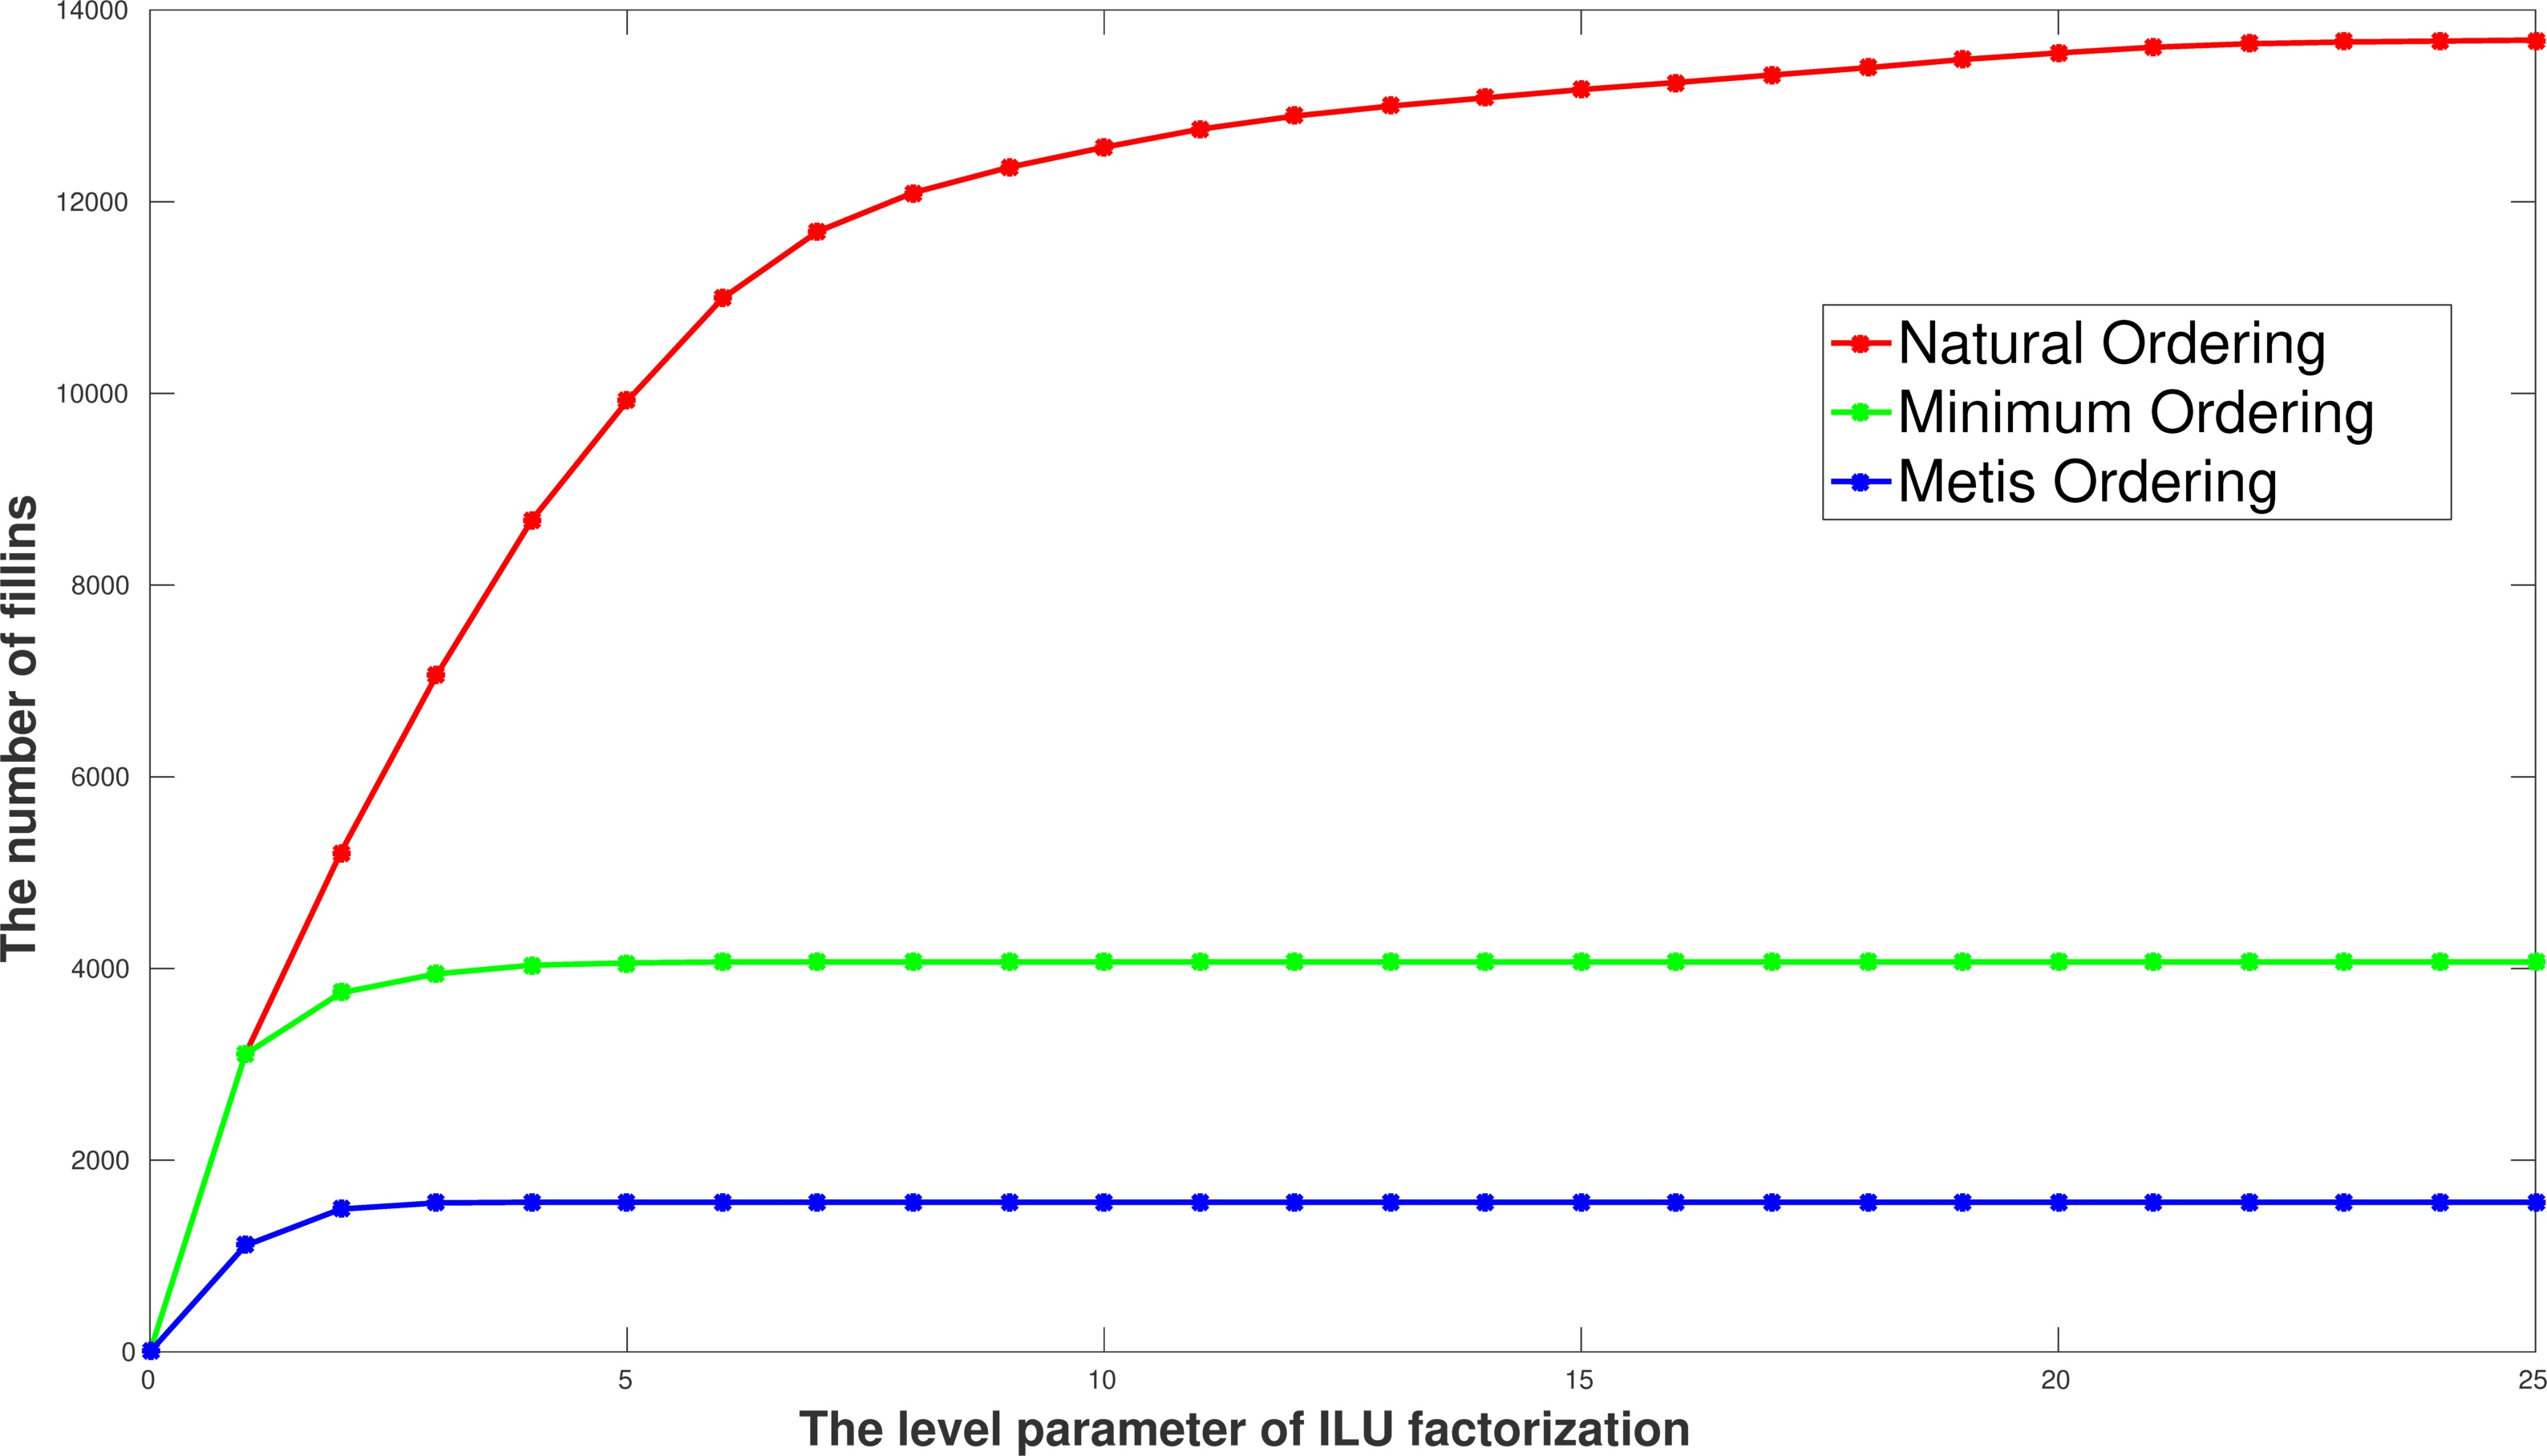
\includegraphics[width=0.9\linewidth]{el_fillins_orderings.jpg}
\caption{The influence of the level parameter for ILU on the number of fill-ins
while three different orderings are employed.
The block size is fixed to $100$.
The matrix is \textit{ex33} and the level parameter changes from $0$ to $25$.
The ordering for coloring is \textit{LFO}.}
\label{el_fillins_orderings}
\end{figure}

\begin{figure}
\centering
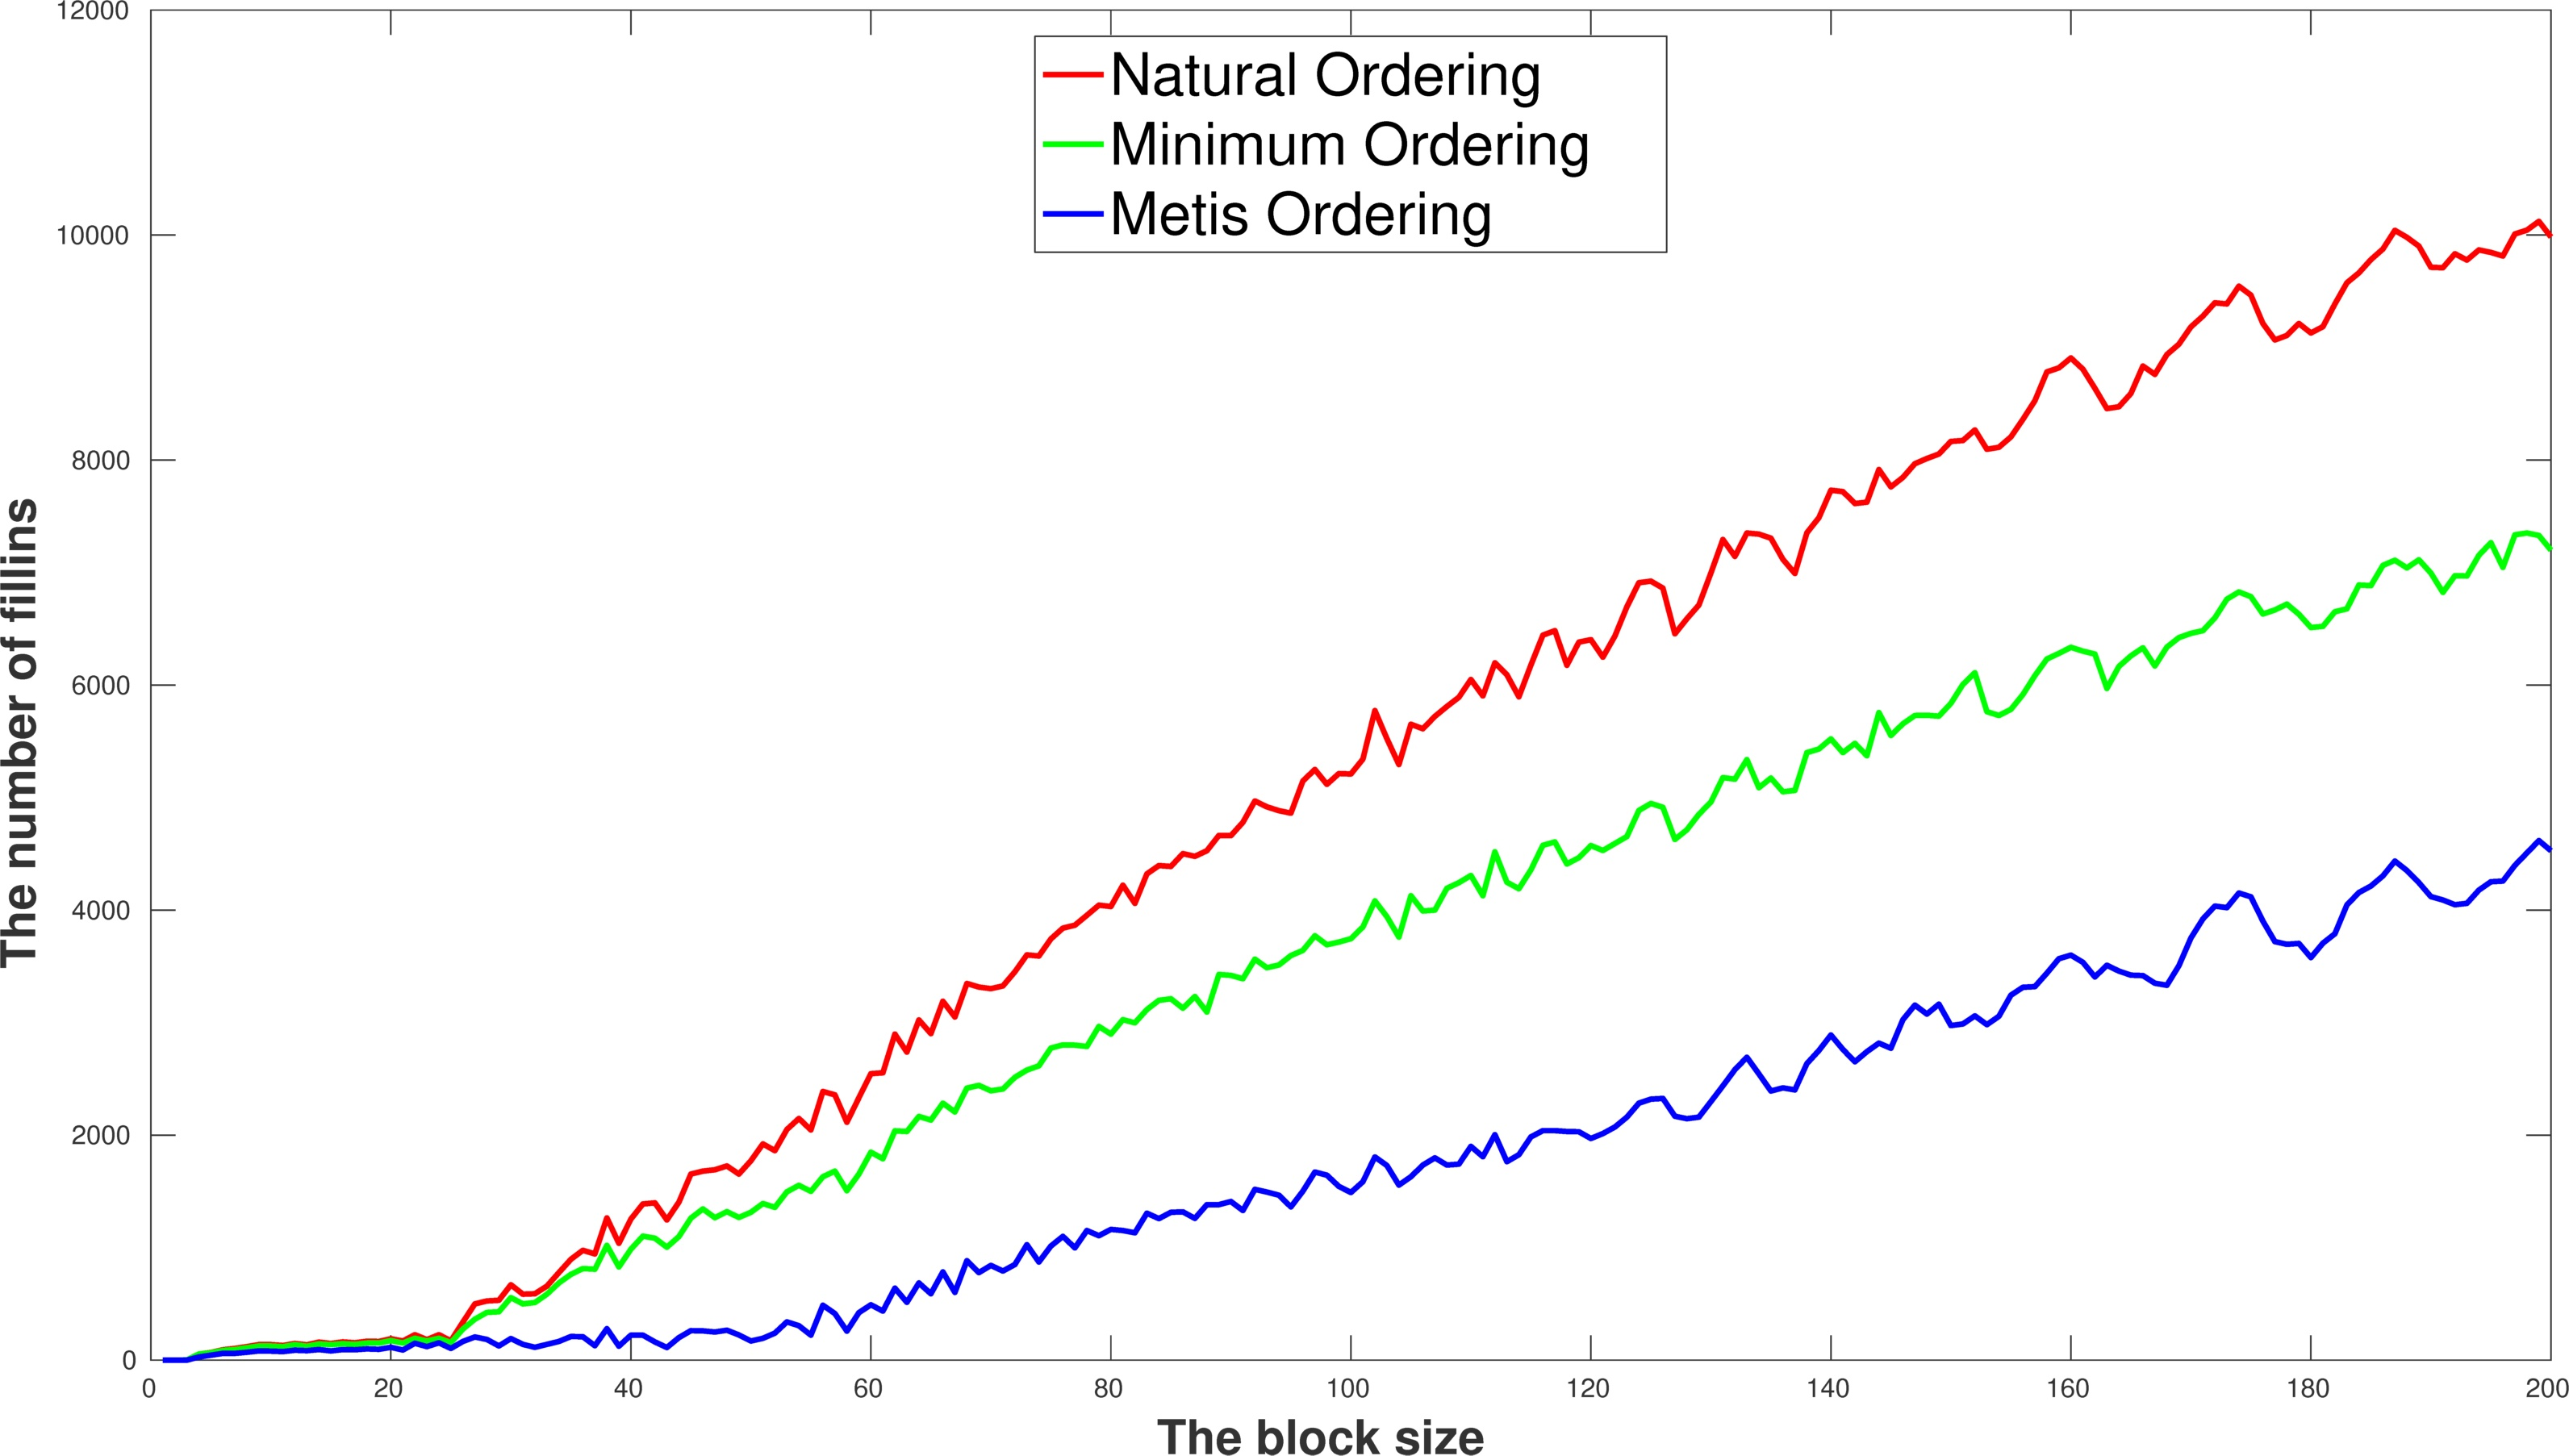
\includegraphics[width=0.9\linewidth]{bls_fillins_orderings.jpg}
\caption{The influence of the block size for sparsification on the number of fill-ins
while three different orderings are employed.
The block size is fixed to $100$.
The matrix is \textit{ex33} and the block size changes from $1$ to $200$.
The ordering for coloring is \textit{LFO}.}
\label{bls_fillins_orderings}
\end{figure}

On the other hand, the coloring has its influence on the number of
additionally required elements. Table~\ref{col-effect}

Here, we did not change any settings other than the ordering of coloring. The ordering for
ILU preconditioning is fixed to the natural ordering.
The block size is $50$ and $10$ and the ILU level is $5$ and $2$ for two matrices
\textit{gyro\_m} and \textit{nos3}, respectively.
The matrix is \textit{gyro\_m}.
\begin{table}
\begin{tabular}{|c|c|c|c|}
\hline
Ordering & Colors & Fill-ins & $|R_a|$ \\\hline
LFO & 34 & 8760 & 66554 \\\hline
SLO & 33 & 8760 & 57760 \\\hline
IDO & 35 & 8760 & 66588 \\\hline
\end{tabular}
\hfill
\begin{tabular}{|c|c|c|c|}
\hline
Ordering & Colors & Fill-ins & $|R_a|$ \\\hline
LFO & 15 & 50 & 394 \\\hline
SLO & 12 & 50 & 384 \\\hline
IDO & 16 & 50 & 436 \\\hline
\end{tabular}
\caption{The effect of coloring on the number of additionally required elements
computed for two matrix \textit{gyro\_m} and \textit{nos3}. }
\label{col-effect}
\end{table}

It can be seen that the number of additionally required elements increases when
the number of colors decreases. This is understood as the number of potentially
required elements are chosen from the non-required elements and added to the required elements
such that number of colors does not increase. Hence, if the number of colors is more,
the freedom of choosing elements gets higher.
As two tables~\ref{ilu-effect} and~\ref{col-effect} shows,
both the ordering of coloring and the ordering of preconditioning affects the number of
additionally required elements. Although smaller number of fill-in increases
the number of additionally required elements, the smaller number of colors
decreases the number of additionally required elements.
This is in contrast to the minimum number of colors which we are searching for,
in the automatic differentiation.
